\chapter {Cortázar, Escher, Bach}
Es posible hacer una comparación directa entre el cuento «Continuidad de los parques» de Julio Cortázar, \emph{Galería de grabados}, de M. C. Escher y el «Canon por tonos» de \emph{La Ofrenda Musical} de J. S. Bach.

En este episodio de la composición de Bach encontramos el Tema Real en una de las múltiples versiones ideadas por el músico alemán a partir del original propuesto por el rey Federico II de Prusia.

\begin{figure}[H]
\begin{center}
\begin{lilypond}[staffsize=16]
\relative c' {
	\key c \minor
	\time 2/4
	c4 es
	g as
	b,4. g'8
	fis4 f
	e es  ~
	es8 d des c
	b a16 g c8 f
	es4 d
	c2 \bar "|."
}
\end{lilypond}
\end{center}
\caption{\emph{«Tema Real» atribuido a Federico II de Prusia.}}
\label{ceb:temareal}
\end{figure}

\noindent Esta versión consiste en variaciones de tipo tanto rítmicas como melódico-armónicas. Estas últimas se destacan por su carácter modulatorio, es decir que el tema, comenzado en do menor, no termina en la tonalidad original sino que en este caso lo hace un tono más arriba, o sea en re menor.

\begin{figure}[H]
\begin{center}
\begin{lilypond}[staffsize=16]
\relative c' {
	\key c \minor
	\time 2/4
	c4 es
	g as
	b,4. g'8
	fis4 f
	e es  ~
	es8 d d d
	cis b16 a d8 g
	f4 e
	d2 \bar "|."
}
\end{lilypond}
\end{center}
\caption{\emph{«Tema Real» modulan, de do menor a re menor.
}$^{\ref{NotaAlPieModula}}$}
\label{ceb:temamodulado}
\end{figure}

\addtocounter{footnote}{1}
\footnotetext[\value{footnote}]{Este tema, tal cual se ve aquí, jamás fue escrito por Bach; lo presentamos sin variaciones rítmicas con respecto al Tema Real para que auditivamente pueda hacerse más fácilmente la comparación desde el punto de vista melódico-armónico exclusivamente.\label{NotaAlPieModula}}

Esta pequeña pieza posee dos voces más: la más grave dibuja un contracanto que posee un mayor dinamismo rítmico que contrasta con el Tema Real; una voz intermedia aparece en el segundo compás imitando al contracanto a distancia de 5ª ascendente. Estas dos voces cumplen un papel decisivo en el proceso modulatorio hacia re menor, ya que sin la intervención de ellas dicho proceso se oiría como forzado. Ahora bien, ¿cual era la intención de Bach al presentar conscientemente una obra que provoque inestabilidad tonal en el oyente? Como en gran medida \emph{La Ofrenda Musical} fue «ofrendada» al rey en forma de enigmas a resolver (\emph{ricercare}, re-buscar), no es difícil ni desatinado afirmar que éste era uno de ellos. La solución a este problema no es complicada: como el oído humano percibe el intervalo de 8ª como ciclo, y al poseer éste seis pasos de tonos, lo que se debe hacer para no quedar tonalmente «descolocado» es ejecutar seis veces seguidas el canon, cada una de ellas un tono más arriba que la vez anterior, y así la última llegaría a la tonalidad inicial. Sin embargo ---más aún si tenemos en cuenta que esta página musical no fue escrita para ningún instrumento en particular--- también es posible leer el siguiente mensaje en esta travesura bachiana: el «Canon por tonos» puede ascender infinitamente\ldots

En \emph{Galería de grabados} encontramos en una galería de arte a dos personas. Una de ellas observa uno de los grabados expuestos. Éste consiste en un barco en el agua, más atrás casas, edificios que se extienden hacia la derecha, en un techo un jovencito parece descansar, más abajo, asomada en un ventanal, una mujer parece observar, siguiendo hacia abajo del ventanal hay un techo que cubre una galería de arte donde hay dos hombres apreciando grabados. Uno de ellos ve uno que consiste en un barco en el agua, más atrás casas, edificios que se extienden hacia la derecha\ldots

En «Continuidad de los parques», el parque, ¿no es la ciudad del grabado de Escher? ; el hombre que lee literatura, ¿no es el hombre que ve el grabado? ; ¿acaso ambos no terminan involucrándose a punto tal que terminan siendo parte de la novela y del grabado respectivamente? ; los dos puntos que encontramos en el párrafo final del cuento, ¿no equivalen a la firma del grabadista holandés, estampada en el centro del espiral que supone su trabajo?

Observemos un poco más el canon de Bach. Dijimos que la voz más grave hace un contracanto que a su vez es imitado por la voz intermedia mientras la voz superior canta el tema real. Cada voz parece tener su rol bien diferenciado. Pero si hilamos más fino empezamos a darnos con ciertas sorpresitas:

\begin{figure}[H]
\begin{center}
\begin{lilypond}[staffsize=16]
global = {
  \key c \minor
  \time 4/4
}

contralto = \relative c' {
  \global
  \clef alto
  R1
  r16 \[ \override NoteHead.color =  #red \override Stem.color = #red \override Beam.color = #red {g bes d g2 f8 e
  f4 ~ f16 b, a}  b \override NoteHead.color =  #black \override Stem.color = #black \override Beam.color = #black c g c d ees4 ~
  ees8 \override NoteHead.color =  #blue \override Stem.color = #blue \override Beam.color = #blue ees[ d c] bes4 ~ bes16[ c bes] \override NoteHead.color =  #black \override Stem.color = #black \override Beam.color = #black a
  g8 aes a4 r8 bes a g
  fis g16 fis g a g f e d e f g e f g\]
}

bajo = \relative c {
  \global
  \clef bass
  r16\[ c ees g c2 bes8 a
  bes4 ~ bes16 e, d e f \override NoteHead.color =  #red \override Stem.color = #red \override Beam.color = #red c f g aes4 ~
  aes8 aes g f ees4 ~ees16 f ees d \override NoteHead.color =  #black \override Stem.color = #black \override Beam.color = #black
  c8 cis d4 r8 \override NoteHead.color =  #blue \override Stem.color = #blue \override Beam.color = #blue ees d c
  b c16 b \override NoteHead.color =  #black \override Stem.color = #black \override Beam.color = #black c d c bes a g a bes c a bes c\]
  d8 c' ~ c bes16 a bes8 g e a16 g
}
\score {
	\new StaffGroup
	<<
		\new Staff {\contralto}
		\new Staff {\bajo}
	>>
}
\end{lilypond}
\end{center}
\caption{\emph{Bach: Canon a la quinta del «Canon por tonos»: Imitación imitada.}}
\label{ceb:imitacion}
\end{figure}

\noindent Con corchetes marcamos la imitación propiamente dicha; en rojo y azul, ¡las otras! ¿Es posible? ¿La voz que imita es imitada? ¿Quién imita a quién?\ldots El tema real, decíamos, es presentado por la voz superior (ver Ejemplo \ref {ceb:completado}).

\begin{figure}[H]
\begin{center}
\begin{lilypond}[staffsize=16]
global = {
	\key c \minor
	\time 4/4
}
soprano = \relative c' {
	\global
	\clef treble
	c4. d8 es e f fis
	g2 aes4 ~ aes16 f des c
	b4 r r g' ~
	g fis2 f4 ~
	f e2 es4 ~
	es d ~ d8 cis b a
	d4 r r
	\override NoteHead.color =  #red
	\override Stem.color = #red
	g ~
	g4 f e2
	\override NoteHead.color =  #black
	\override Stem.color = #black
}
alto = \relative c' {
  \global
  \clef alto
  R1
  r16 g bes d g2 f8 e
  f4 ~ f16 b, a b c g c d es4 ~
  es8 es d c bes4 ~ bes16 c bes a
  g8 aes a4 r8 bes a g
  fis g16 fis g a g f e d e f g e f g
  \autoBeamOff
  a8 
  \autoBeamOn
  \override NoteHead.color =  #red
  \override Stem.color = #red
  \override Beam.color = #red
  g' ~ g f16 e
  \override NoteHead.color =  #black
  \override Stem.color = #black
  \override Beam.color = #black
  f8 d b e16 d
  cis8 d16 e f8 gis, a4 r
}
\score {
	\new StaffGroup
	<<
		\new Staff = "sop" {\soprano}
		\new Staff = "alt" {\alto}
	>>
}
\end{lilypond}
\end{center}
\caption{\emph{El Tema Real completado y anticipado.}}
\label{ceb:completado}
\end{figure}

¿Es presentado solamente por la voz superior? El astuto silencio introducido en el séptimo compás hace callar a la voz encargada de hacer oír el tema real cediendo en ese momento la tarea a la voz intermedia, la cual \emph{completa} la melodía con una rítmica que se acerca a la del original de Federico II. Sin embargo, poco después, la voz superior también completa el canto dado. Por lo tanto lo que la segunda voz hace puede entenderse también como una \emph{anticipación}, que, no olvidemos, fue a la vez anunciada por la tercera voz un compás atrás (\emph{«Un diálogo anhelante corría por las páginas como un arroyo de serpientes, y se sentía que \emph{todo estaba decidido desde siempre}. [\ldots]Los perros no debían ladrar, y no ladraron. El mayordomo no estaría a esa hora, y no estaba.»)}.

Esta ambigüedad en los límites, ¿no es la misma de la ciudad escheriana o del parque cortazariano?

Podemos aquí, a modo de curiosidad, hacer mención al hecho de que es posible ejecutar «infinitamente» el canon por tonos de Bach. Robert Shepard, psicólogo, ideó un artificio por el cual se logra dar la ilusión de que se asciende sin realmente hacerlo. El método consiste en, dada una escala ascendente, ejecutarla con intensidades decrecientes y, simultáneamente, hacer oír la misma escala una octava más baja, pero con intensidades ascendentes. El resultado, como dijimos, es que parece subir, pero no sube, lo que da la posibilidad de repetir el proceso \emph{ad infinitum}.

\begin{figure}[H]
\begin{center}
\begin{lilypond}[notime,staffsize=16]
\relative c' {
	\time 6/4
	<<
	{\repeat volta 2 {
	\once \set fontSize = #3
	c' 
	\once \set fontSize = #2
	d 
	\once \set fontSize = #1
	e 
	\once \set fontSize = #0
	fis 
	\once \set fontSize = #-1
	gis 
	\once \set fontSize = #-2
	ais } 
	\once \set fontSize = #-3
	c}
	\\ 
	{
	\once \set fontSize = #-3
	c,,4 
	\once \set fontSize = #-2
	d 
	\once \set fontSize = #-1
	e 
	\once \set fontSize = #0
	fis 
	\once \set fontSize = #1
	gis 
	\once \set fontSize = #2
	ais 
	\once \set fontSize = #3
	c}
>>
}
\end{lilypond}
\end{center}
\caption{\emph{Tonos de Shepard.}}
\label{ceb:shepard}
\end{figure}

Escher habla de las artes plásticas con las artes plásticas; Cortázar habla de la literatura con la literatura; ¿Bach habla de la música con la música?

Es posible hacer una comparación directa entre el cuento «Continuidad de los parques» de Julio Cortázar, \emph{Galería de grabados}, de M. C. Escher y el «Canon por tonos» de \emph{La Ofrenda Musical} de J. S. Bach.

%Apéndice
\newpage
\section {Apéndice indispensable}
\subsection {Canon por tonos}
\noindent \textsc{J. S. Bach}
\begin{figure}[H]
\begin{center}
\begin{lilypond}[staffsize=14]
global = {
  \key c \minor
  \time 4/4
}

soprano = \relative c' {
  \global
  \clef treble
  c4. d8 es e f fis
  g2 aes4 ~ aes16 f des c
  b4 r r g' ~
  g fis2 f4 ~
  f e2 es4 ~
  es d ~ d8 cis b a
  d4 r r g ~
  g4 f e2
  \bar "||"
  \key d \minor
  d4. e8 d fis g gis
}

alto = \relative c' {
  \global
  \clef alto
  R1
  r16 g bes d g2 f8 e
  f4 ~ f16 b, a b c g c d ees4 ~
  ees8 ees d c bes4 ~ bes16 c bes a
  g8 aes a4 r8 bes a g
  fis g16 fis g a g f e d e f g e f g
  a8 g'4 f16 e f8 d b e16 d
  cis8 d16 e f8 gis, a4 r
  \bar "||"
  \key d \minor
  r8 a ~ a16 c b a gis a b c d f e d
}

bajo = \relative c {
  \global
  \clef bass
  r16 c ees g c2 bes8 a
  bes4 ~ bes16 e, d e f c f g aes4 ~
  aes8 aes g f ees4 ~ees16 f ees d
  c8 cis d4 r8 ees d c
  b c16 b c d c bes a g a bes c a bes c
  d8 c'4 bes16 a bes8 g e a16 g
  fis8 g16 a bes8 cis, d4 r
  r8 d ~ d16 f e d cis d e f g bes a g
  \bar "||"
  \key d \minor
  f d f a d2 c8 b
}

\score {
  \new StaffGroup
  <<
    \soprano
    \alto
    \bajo
  >>
}
\end{lilypond}
\end{center}
\caption{\emph{J. S. Bach: «Canon por Tonos» de la \emph{Ofrenda Musical} (1747).}}
\label{ceb:ofrenda}
\end{figure}
\newpage
\subsection {Galería de grabados}
\noindent \textsc{M. C. Escher}
\vspace{2cm}
\begin{figure}[H]
  \centering
    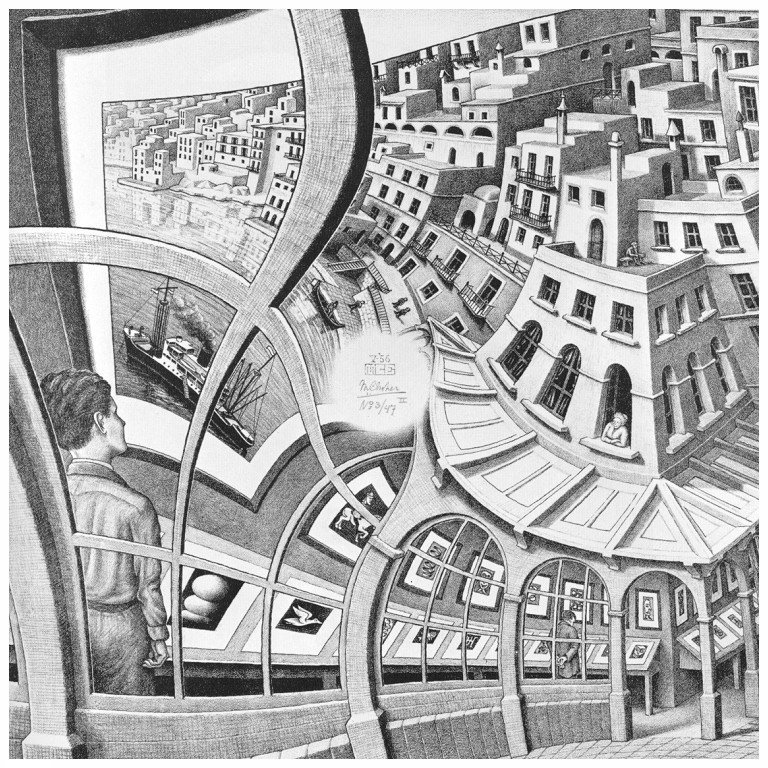
\includegraphics[width=1\textwidth]{c-ceb}
  \caption{\emph{M. C. Escher, \emph{Galería de grabados}  (1956).}}
  \label{ceb:galeria}
\end{figure}
\newpage
\subsection{Continuidad de los parques}
\begin{flushright}
\textsc{Julio Cortázar}
\end{flushright}
\bigskip

\begin {quotation}
\textit {Había empezado a leer la novela unos días antes. La abandonó por negocios urgentes, volvió a abrirla cuando regresaba en tren a la finca; se dejaba interesar lentamente por la trama, por el dibujo de los personajes. Esa tarde, después de escribir una carta a su apoderado y discutir con el mayordomo una cuestión de aparcerías, volvió al libro en la tranquilidad del estudio que miraba hacia el parque de los robles. Arrellanado en su sillón favorito, de espaldas a la puerta que lo hubiera molestado como una irritante posibilidad de intrusiones, dejó que su mano izquierda acariciara una y otra vez el terciopelo verde y se puso a leer los últimos capítulos. Su memoria retenía sin esfuerzo los nombres y las imágenes de los protagonistas; la ilusión novelesca lo ganó casi enseguida. Gozaba del placer casi perverso de irse desgajando línea a línea de lo que lo rodeaba, y sentir que a la vez su cabeza descansaba cómodamente en el terciopelo del alto respaldo, que los cigarrillos seguían al alcance de la mano, que más allá de los ventanales danzaba el aire del atardecer bajo los robles. Palabra a palabra, absorbido por la sórdida disyuntiva de los héroes, dejándose ir hacia las imágenes que se concertaban y adquirían color y movimiento, fue testigo del último encuentro en la cabaña del monte. Primero entraba la mujer, recelosa; ahora llegaba el amante, lastimada la cara por el chicotazo de una rama. Admirablemente restañaba ella la sangre con sus besos, pero él rechazaba las caricias, no había venido para repetir las ceremonias de una pasión secreta, protegida por un mundo de hojas secas y senderos furtivos. El puñal se entibiaba contra su pecho, y debajo latía la libertad agazapada. Un diálogo anhelante corría por las páginas como un arroyo de serpientes, y se sentía que todo estaba decidido desde siempre. Hasta esas caricia que enredaba el cuerpo del amante como queriendo retenerlo y disuadirlo, dibujaban abominablemente la figura de otro cuerpo que era necesario destruir. Nada había sido olvidado: coartadas, azares, posibles errores. A partir de esa hora cada instante tenía su empleo minuciosamente atribuido. El doble repaso despiadado se interrumpía apenas para que una mano acariciara una mejilla. Empezaba a anochecer.}

\textit{Sin mirarse ya, atados rígidamente a la tarea que los esperaba, se separaron en la puerta de la cabaña. Ella debía seguir por la senda que iba al norte. Desde la senda opuesta él se volvió un instante para verla correr con el pelo suelto. Corrió a su vez, parapetándose en los árboles y los setos, hasta distinguir en la bruma malva del crepúsculo la alameda que llevaba a la casa. Los perros no debían ladrar, y no ladraron. El mayordomo no estaría a esa hora, y no estaba. Subió los tres peldaños del porche y entró. Desde la sangre galopando en sus oídos le llegaban las palabras de la mujer: primero una sala azul, después una galería, una escalera alfombrada. En lo alto, dos puertas. Nadie en la primera habitación, nadie en la segunda. La puerta del salón, y entonces el puñal en la mano, la luz de los ventanales, el alto respaldo de un sillón de terciopelo verde, la cabeza del hombre en el sillón leyendo una novela.}
\end{quotation}
